\documentclass[1p]{elsarticle_modified}
%\bibliographystyle{elsarticle-num}

%\usepackage[colorlinks]{hyperref}
%\usepackage{abbrmath_seonhwa} %\Abb, \Ascr, \Acal ,\Abf, \Afrak
\usepackage{amsfonts}
\usepackage{amssymb}
\usepackage{amsmath}
\usepackage{amsthm}
\usepackage{scalefnt}
\usepackage{amsbsy}
\usepackage{kotex}
\usepackage{caption}
\usepackage{subfig}
\usepackage{color}
\usepackage{graphicx}
\usepackage{xcolor} %% white, black, red, green, blue, cyan, magenta, yellow
\usepackage{float}
\usepackage{setspace}
\usepackage{hyperref}

\usepackage{tikz}
\usetikzlibrary{arrows}

\usepackage{multirow}
\usepackage{array} % fixed length table
\usepackage{hhline}

%%%%%%%%%%%%%%%%%%%%%
\makeatletter
\renewcommand*\env@matrix[1][\arraystretch]{%
	\edef\arraystretch{#1}%
	\hskip -\arraycolsep
	\let\@ifnextchar\new@ifnextchar
	\array{*\c@MaxMatrixCols c}}
\makeatother %https://tex.stackexchange.com/questions/14071/how-can-i-increase-the-line-spacing-in-a-matrix
%%%%%%%%%%%%%%%

\usepackage[normalem]{ulem}

\newcommand{\msout}[1]{\ifmmode\text{\sout{\ensuremath{#1}}}\else\sout{#1}\fi}
%SOURCE: \msout is \stkout macro in https://tex.stackexchange.com/questions/20609/strikeout-in-math-mode

\newcommand{\cancel}[1]{
	\ifmmode
	{\color{red}\msout{#1}}
	\else
	{\color{red}\sout{#1}}
	\fi
}

\newcommand{\add}[1]{
	{\color{blue}\uwave{#1}}
}

\newcommand{\replace}[2]{
	\ifmmode
	{\color{red}\msout{#1}}{\color{blue}\uwave{#2}}
	\else
	{\color{red}\sout{#1}}{\color{blue}\uwave{#2}}
	\fi
}

\newcommand{\Sol}{\mathcal{S}} %segment
\newcommand{\D}{D} %diagram
\newcommand{\A}{\mathcal{A}} %arc


%%%%%%%%%%%%%%%%%%%%%%%%%%%%%5 test

\def\sl{\operatorname{\textup{SL}}(2,\Cbb)}
\def\psl{\operatorname{\textup{PSL}}(2,\Cbb)}
\def\quan{\mkern 1mu \triangleright \mkern 1mu}

\theoremstyle{definition}
\newtheorem{thm}{Theorem}[section]
\newtheorem{prop}[thm]{Proposition}
\newtheorem{lem}[thm]{Lemma}
\newtheorem{ques}[thm]{Question}
\newtheorem{cor}[thm]{Corollary}
\newtheorem{defn}[thm]{Definition}
\newtheorem{exam}[thm]{Example}
\newtheorem{rmk}[thm]{Remark}
\newtheorem{alg}[thm]{Algorithm}

\newcommand{\I}{\sqrt{-1}}
\begin{document}

%\begin{frontmatter}
%
%\title{Boundary parabolic representations of knots up to 8 crossings}
%
%%% Group authors per affiliation:
%\author{Yunhi Cho} 
%\address{Department of Mathematics, University of Seoul, Seoul, Korea}
%\ead{yhcho@uos.ac.kr}
%
%
%\author{Seonhwa Kim} %\fnref{s_kim}}
%\address{Center for Geometry and Physics, Institute for Basic Science, Pohang, 37673, Korea}
%\ead{ryeona17@ibs.re.kr}
%
%\author{Hyuk Kim}
%\address{Department of Mathematical Sciences, Seoul National University, Seoul 08826, Korea}
%\ead{hyukkim@snu.ac.kr}
%
%\author{Seokbeom Yoon}
%\address{Department of Mathematical Sciences, Seoul National University, Seoul, 08826,  Korea}
%\ead{sbyoon15@snu.ac.kr}
%
%\begin{abstract}
%We find all boundary parabolic representation of knots up to 8 crossings.
%
%\end{abstract}
%\begin{keyword}
%    \MSC[2010] 57M25 
%\end{keyword}
%
%\end{frontmatter}

%\linenumbers
%\tableofcontents
%
\newcommand\colored[1]{\textcolor{white}{\rule[-0.35ex]{0.8em}{1.4ex}}\kern-0.8em\color{red} #1}%
%\newcommand\colored[1]{\textcolor{white}{ #1}\kern-2.17ex	\textcolor{white}{ #1}\kern-1.81ex	\textcolor{white}{ #1}\kern-2.15ex\color{red}#1	}

{\Large $\underline{11n_{110}~(K11n_{110})}$}

\setlength{\tabcolsep}{10pt}
\renewcommand{\arraystretch}{1.6}
\vspace{1cm}\begin{tabular}{m{100pt}>{\centering\arraybackslash}m{274pt}}
\multirow{5}{120pt}{
	\centering
	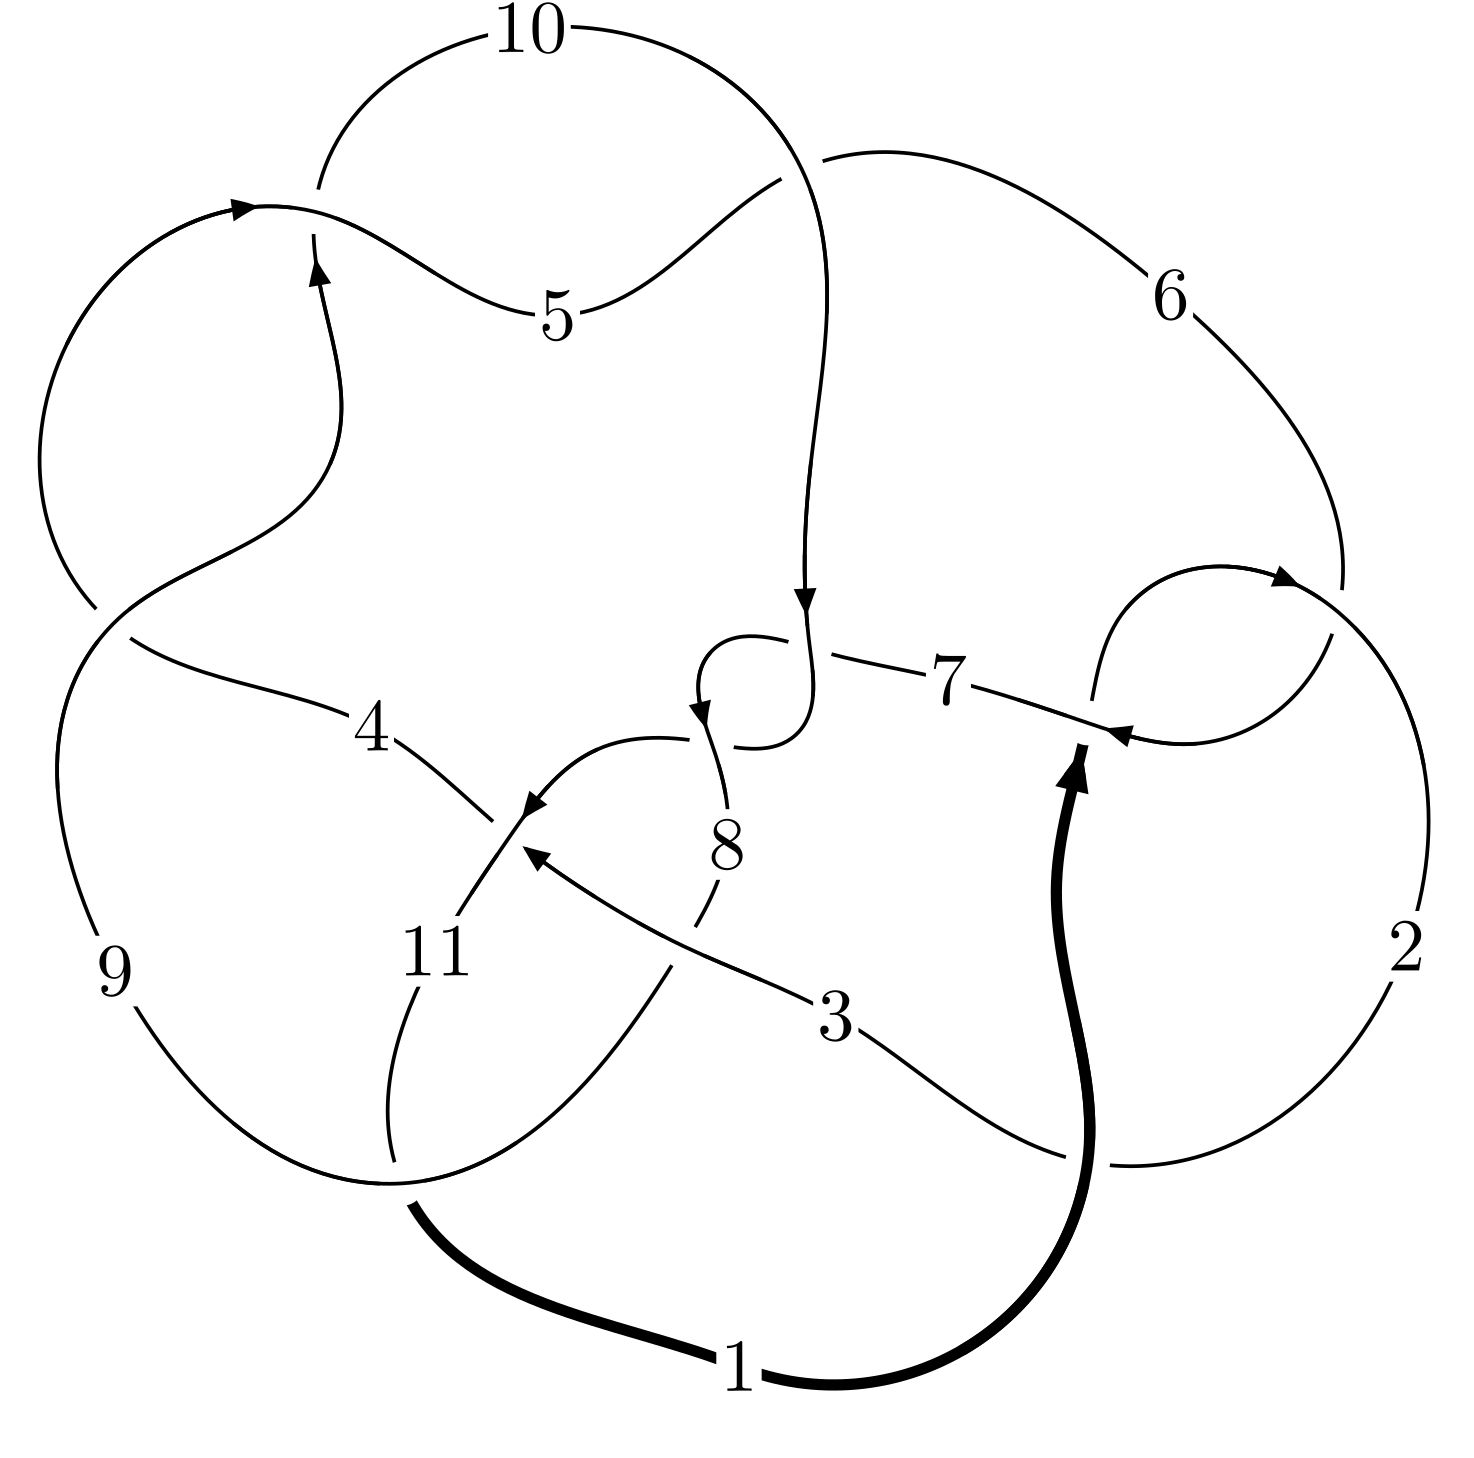
\includegraphics[width=112pt]{../../../GIT/diagram.site/Diagrams/png/726_11n_110.png}\\
\ \ \ A knot diagram\footnotemark}&
\allowdisplaybreaks
\textbf{Linearized knot diagam} \\
\cline{2-2}
 &
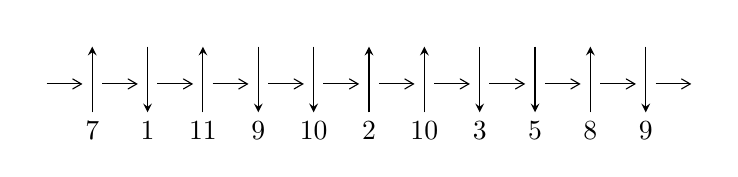
\begin{tikzpicture}[x=20pt, y=17pt]
	% nodes
	\node (C0) at (0, 0) {};
	\node (C1) at (1, 0) {};
	\node (C1U) at (1, +1) {};
	\node (C1D) at (1, -1) {7};

	\node (C2) at (2, 0) {};
	\node (C2U) at (2, +1) {};
	\node (C2D) at (2, -1) {1};

	\node (C3) at (3, 0) {};
	\node (C3U) at (3, +1) {};
	\node (C3D) at (3, -1) {11};

	\node (C4) at (4, 0) {};
	\node (C4U) at (4, +1) {};
	\node (C4D) at (4, -1) {9};

	\node (C5) at (5, 0) {};
	\node (C5U) at (5, +1) {};
	\node (C5D) at (5, -1) {10};

	\node (C6) at (6, 0) {};
	\node (C6U) at (6, +1) {};
	\node (C6D) at (6, -1) {2};

	\node (C7) at (7, 0) {};
	\node (C7U) at (7, +1) {};
	\node (C7D) at (7, -1) {10};

	\node (C8) at (8, 0) {};
	\node (C8U) at (8, +1) {};
	\node (C8D) at (8, -1) {3};

	\node (C9) at (9, 0) {};
	\node (C9U) at (9, +1) {};
	\node (C9D) at (9, -1) {5};

	\node (C10) at (10, 0) {};
	\node (C10U) at (10, +1) {};
	\node (C10D) at (10, -1) {8};

	\node (C11) at (11, 0) {};
	\node (C11U) at (11, +1) {};
	\node (C11D) at (11, -1) {9};
	\node (C12) at (12, 0) {};

	% arrows
	\draw[->,>={angle 60}]
	(C0) edge (C1) (C1) edge (C2) (C2) edge (C3) (C3) edge (C4) (C4) edge (C5) (C5) edge (C6) (C6) edge (C7) (C7) edge (C8) (C8) edge (C9) (C9) edge (C10) (C10) edge (C11) (C11) edge (C12) ;	\draw[->,>=stealth]
	(C1D) edge (C1U) (C2U) edge (C2D) (C3D) edge (C3U) (C4U) edge (C4D) (C5U) edge (C5D) (C6D) edge (C6U) (C7D) edge (C7U) (C8U) edge (C8D) (C9U) edge (C9D) (C10D) edge (C10U) (C11U) edge (C11D) ;
	\end{tikzpicture} \\
\hhline{~~} \\& 
\textbf{Solving Sequence} \\ \cline{2-2} 
 &
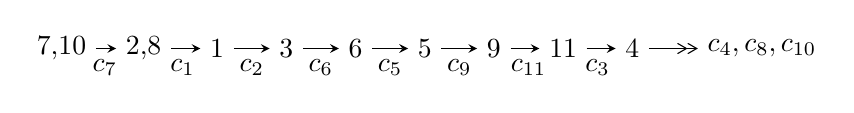
\begin{tikzpicture}[x=25pt, y=7pt]
	% node
	\node (A0) at (-1/8, 0) {7,10};
	\node (A1) at (17/16, 0) {2,8};
	\node (A2) at (17/8, 0) {1};
	\node (A3) at (25/8, 0) {3};
	\node (A4) at (33/8, 0) {6};
	\node (A5) at (41/8, 0) {5};
	\node (A6) at (49/8, 0) {9};
	\node (A7) at (57/8, 0) {11};
	\node (A8) at (65/8, 0) {4};
	\node (C1) at (1/2, -1) {$c_{7}$};
	\node (C2) at (13/8, -1) {$c_{1}$};
	\node (C3) at (21/8, -1) {$c_{2}$};
	\node (C4) at (29/8, -1) {$c_{6}$};
	\node (C5) at (37/8, -1) {$c_{5}$};
	\node (C6) at (45/8, -1) {$c_{9}$};
	\node (C7) at (53/8, -1) {$c_{11}$};
	\node (C8) at (61/8, -1) {$c_{3}$};
	\node (A9) at (10, 0) {$c_{4},c_{8},c_{10}$};

	% edge
	\draw[->,>=stealth]	
	(A0) edge (A1) (A1) edge (A2) (A2) edge (A3) (A3) edge (A4) (A4) edge (A5) (A5) edge (A6) (A6) edge (A7) (A7) edge (A8) ;
	\draw[->>,>={angle 60}]	
	(A8) edge (A9);
\end{tikzpicture} \\ 

\end{tabular} \\

\footnotetext{
The image of knot diagram is generated by the software ``\textbf{Draw programme}" developed by Andrew Bartholomew(\url{http://www.layer8.co.uk/maths/draw/index.htm\#Running-draw}), where we modified some parts for our purpose(\url{https://github.com/CATsTAILs/LinksPainter}).
}\phantom \\ \newline 
\centering \textbf{Ideals for irreducible components\footnotemark of $X_{\text{par}}$} 
 
\begin{align*}
I^u_{1}&=\langle 
-5.24577\times10^{42} u^{29}-3.23671\times10^{42} u^{28}+\cdots+1.72502\times10^{43} b+9.64831\times10^{44},\\
\phantom{I^u_{1}}&\phantom{= \langle  }-1.04908\times10^{45} u^{29}-2.98068\times10^{44} u^{28}+\cdots+2.46678\times10^{45} a+3.12089\times10^{47},\\
\phantom{I^u_{1}}&\phantom{= \langle  }u^{30}-20 u^{28}+\cdots-702 u+143\rangle \\
I^u_{2}&=\langle 
2 u^9+u^8-8 u^7-3 u^6+12 u^5+4 u^4-5 u^3-4 u^2+b+2 u+1,\\
\phantom{I^u_{2}}&\phantom{= \langle  }u^9+u^8-3 u^7-3 u^6+2 u^5+3 u^4+4 u^3+a-3 u-1,\\
\phantom{I^u_{2}}&\phantom{= \langle  }u^{10}+u^9-4 u^8-4 u^7+6 u^6+7 u^5-2 u^4-6 u^3- u^2+2 u+1\rangle \\
\\
\end{align*}
\raggedright * 2 irreducible components of $\dim_{\mathbb{C}}=0$, with total 40 representations.\\
\footnotetext{All coefficients of polynomials are rational numbers. But the coefficients are sometimes approximated in decimal forms when there is not enough margin.}
\newpage
\renewcommand{\arraystretch}{1}
\centering \section*{I. $I^u_{1}= \langle -5.25\times10^{42} u^{29}-3.24\times10^{42} u^{28}+\cdots+1.73\times10^{43} b+9.65\times10^{44},\;-1.05\times10^{45} u^{29}-2.98\times10^{44} u^{28}+\cdots+2.47\times10^{45} a+3.12\times10^{47},\;u^{30}-20 u^{28}+\cdots-702 u+143 \rangle$}
\flushleft \textbf{(i) Arc colorings}\\
\begin{tabular}{m{7pt} m{180pt} m{7pt} m{180pt} }
\flushright $a_{7}=$&$\begin{pmatrix}1\\0\end{pmatrix}$ \\
\flushright $a_{10}=$&$\begin{pmatrix}0\\u\end{pmatrix}$ \\
\flushright $a_{2}=$&$\begin{pmatrix}0.425284 u^{29}+0.120833 u^{28}+\cdots+435.751 u-126.517\\0.304099 u^{29}+0.187633 u^{28}+\cdots+228.271 u-55.9316\end{pmatrix}$ \\
\flushright $a_{8}=$&$\begin{pmatrix}1\\- u^2\end{pmatrix}$ \\
\flushright $a_{1}=$&$\begin{pmatrix}0.121185 u^{29}-0.0668003 u^{28}+\cdots+207.480 u-70.5855\\0.304099 u^{29}+0.187633 u^{28}+\cdots+228.271 u-55.9316\end{pmatrix}$ \\
\flushright $a_{3}=$&$\begin{pmatrix}0.106102 u^{29}-0.0778641 u^{28}+\cdots+210.361 u-79.9957\\0.135922 u^{29}+0.0365756 u^{28}+\cdots+136.153 u-36.2204\end{pmatrix}$ \\
\flushright $a_{6}=$&$\begin{pmatrix}-0.232141 u^{29}-0.191193 u^{28}+\cdots-134.653 u+22.1188\\-0.164756 u^{29}-0.170846 u^{28}+\cdots-70.5588 u+6.95079\end{pmatrix}$ \\
\flushright $a_{5}=$&$\begin{pmatrix}-0.232141 u^{29}-0.191193 u^{28}+\cdots-134.653 u+22.1188\\-0.0393575 u^{29}-0.0958610 u^{28}+\cdots+30.4623 u-20.3898\end{pmatrix}$ \\
\flushright $a_{9}=$&$\begin{pmatrix}0.218809 u^{29}+0.241071 u^{28}+\cdots+63.2104 u+9.67970\\-0.0214735 u^{29}+0.132358 u^{28}+\cdots-126.031 u+47.6240\end{pmatrix}$ \\
\flushright $a_{11}=$&$\begin{pmatrix}u\\- u^3+u\end{pmatrix}$ \\
\flushright $a_{4}=$&$\begin{pmatrix}0.186030 u^{29}-0.0243156 u^{28}+\cdots+264.074 u-88.9655\\0.190051 u^{29}+0.0781916 u^{28}+\cdots+163.704 u-37.5328\end{pmatrix}$\\ \flushright $a_{4}=$&$\begin{pmatrix}0.186030 u^{29}-0.0243156 u^{28}+\cdots+264.074 u-88.9655\\0.190051 u^{29}+0.0781916 u^{28}+\cdots+163.704 u-37.5328\end{pmatrix}$\\&\end{tabular}
\flushleft \textbf{(ii) Obstruction class $= -1$}\\~\\
\flushleft \textbf{(iii) Cusp Shapes $= -1.06625 u^{29}-0.645061 u^{28}+\cdots-715.257 u+115.725$}\\~\\
\newpage\renewcommand{\arraystretch}{1}
\flushleft \textbf{(iv) u-Polynomials at the component}\newline \\
\begin{tabular}{m{50pt}|m{274pt}}
Crossings & \hspace{64pt}u-Polynomials at each crossing \\
\hline $$\begin{aligned}c_{1},c_{6}\end{aligned}$$&$\begin{aligned}
&u^{30}+3 u^{28}+\cdots+6 u+1
\end{aligned}$\\
\hline $$\begin{aligned}c_{2}\end{aligned}$$&$\begin{aligned}
&u^{30}+6 u^{29}+\cdots+4 u+1
\end{aligned}$\\
\hline $$\begin{aligned}c_{3}\end{aligned}$$&$\begin{aligned}
&u^{30}+u^{29}+\cdots-5 u+1
\end{aligned}$\\
\hline $$\begin{aligned}c_{4},c_{5},c_{9}\end{aligned}$$&$\begin{aligned}
&u^{30}+u^{27}+\cdots-4 u+19
\end{aligned}$\\
\hline $$\begin{aligned}c_{7},c_{10}\end{aligned}$$&$\begin{aligned}
&u^{30}-20 u^{28}+\cdots+702 u+143
\end{aligned}$\\
\hline $$\begin{aligned}c_{8}\end{aligned}$$&$\begin{aligned}
&u^{30}+u^{29}+\cdots- u+3
\end{aligned}$\\
\hline $$\begin{aligned}c_{11}\end{aligned}$$&$\begin{aligned}
&u^{30}-4 u^{29}+\cdots-14 u+1
\end{aligned}$\\
\hline
\end{tabular}\\~\\
\newpage\renewcommand{\arraystretch}{1}
\flushleft \textbf{(v) Riley Polynomials at the component}\newline \\
\begin{tabular}{m{50pt}|m{274pt}}
Crossings & \hspace{64pt}Riley Polynomials at each crossing \\
\hline $$\begin{aligned}c_{1},c_{6}\end{aligned}$$&$\begin{aligned}
&y^{30}+6 y^{29}+\cdots+4 y+1
\end{aligned}$\\
\hline $$\begin{aligned}c_{2}\end{aligned}$$&$\begin{aligned}
&y^{30}+42 y^{29}+\cdots+124 y+1
\end{aligned}$\\
\hline $$\begin{aligned}c_{3}\end{aligned}$$&$\begin{aligned}
&y^{30}-27 y^{29}+\cdots+89 y+1
\end{aligned}$\\
\hline $$\begin{aligned}c_{4},c_{5},c_{9}\end{aligned}$$&$\begin{aligned}
&y^{30}+30 y^{28}+\cdots+5798 y+361
\end{aligned}$\\
\hline $$\begin{aligned}c_{7},c_{10}\end{aligned}$$&$\begin{aligned}
&y^{30}-40 y^{29}+\cdots-169052 y+20449
\end{aligned}$\\
\hline $$\begin{aligned}c_{8}\end{aligned}$$&$\begin{aligned}
&y^{30}+y^{29}+\cdots+149 y+9
\end{aligned}$\\
\hline $$\begin{aligned}c_{11}\end{aligned}$$&$\begin{aligned}
&y^{30}+30 y^{29}+\cdots-30 y+1
\end{aligned}$\\
\hline
\end{tabular}\\~\\
\newpage\flushleft \textbf{(vi) Complex Volumes and Cusp Shapes}
$$\begin{array}{c|c|c}  
\text{Solutions to }I^u_{1}& \I (\text{vol} + \sqrt{-1}CS) & \text{Cusp shape}\\
 \hline 
\begin{aligned}
u &= \phantom{-}0.451767 + 0.791950 I \\
a &= -0.695737 + 0.012247 I \\
b &= -0.129301 + 0.865185 I\end{aligned}
 & -0.95851 - 2.62649 I & -5.25510 + 4.40076 I \\ \hline\begin{aligned}
u &= \phantom{-}0.451767 - 0.791950 I \\
a &= -0.695737 - 0.012247 I \\
b &= -0.129301 - 0.865185 I\end{aligned}
 & -0.95851 + 2.62649 I & -5.25510 - 4.40076 I \\ \hline\begin{aligned}
u &= \phantom{-}0.898711 + 0.095581 I \\
a &= -0.211923 + 1.074670 I \\
b &= -0.472373 + 1.278930 I\end{aligned}
 & \phantom{-}0.32537 - 4.54381 I & \phantom{-}1.91240 + 4.46685 I \\ \hline\begin{aligned}
u &= \phantom{-}0.898711 - 0.095581 I \\
a &= -0.211923 - 1.074670 I \\
b &= -0.472373 - 1.278930 I\end{aligned}
 & \phantom{-}0.32537 + 4.54381 I & \phantom{-}1.91240 - 4.46685 I \\ \hline\begin{aligned}
u &= -0.796766 + 0.348460 I \\
a &= -1.49520 + 0.87151 I \\
b &= \phantom{-}0.307391 - 0.308073 I\end{aligned}
 & \phantom{-}1.43336 - 3.12326 I & \phantom{-}2.11949 + 6.95210 I \\ \hline\begin{aligned}
u &= -0.796766 - 0.348460 I \\
a &= -1.49520 - 0.87151 I \\
b &= \phantom{-}0.307391 + 0.308073 I\end{aligned}
 & \phantom{-}1.43336 + 3.12326 I & \phantom{-}2.11949 - 6.95210 I \\ \hline\begin{aligned}
u &= \phantom{-}1.162640 + 0.268770 I \\
a &= \phantom{-}0.570691 - 0.011630 I \\
b &= \phantom{-}0.324375 - 0.250772 I\end{aligned}
 & -2.62675 - 0.08468 I & -4.72619 - 2.64005 I \\ \hline\begin{aligned}
u &= \phantom{-}1.162640 - 0.268770 I \\
a &= \phantom{-}0.570691 + 0.011630 I \\
b &= \phantom{-}0.324375 + 0.250772 I\end{aligned}
 & -2.62675 + 0.08468 I & -4.72619 + 2.64005 I \\ \hline\begin{aligned}
u &= -0.971060 + 0.777102 I \\
a &= -0.21574 + 1.45380 I \\
b &= \phantom{-}0.344838 + 0.890194 I\end{aligned}
 & \phantom{-}1.65136 - 1.24421 I & \phantom{-}1.024611 - 0.505616 I \\ \hline\begin{aligned}
u &= -0.971060 - 0.777102 I \\
a &= -0.21574 - 1.45380 I \\
b &= \phantom{-}0.344838 - 0.890194 I\end{aligned}
 & \phantom{-}1.65136 + 1.24421 I & \phantom{-}1.024611 + 0.505616 I\\
 \hline 
 \end{array}$$\newpage$$\begin{array}{c|c|c}  
\text{Solutions to }I^u_{1}& \I (\text{vol} + \sqrt{-1}CS) & \text{Cusp shape}\\
 \hline 
\begin{aligned}
u &= \phantom{-}0.484306 + 0.368077 I \\
a &= \phantom{-}0.08679 - 1.82883 I \\
b &= -0.943336 - 0.363298 I\end{aligned}
 & \phantom{-}3.55287 + 0.89069 I & \phantom{-}4.27167 - 0.33793 I \\ \hline\begin{aligned}
u &= \phantom{-}0.484306 - 0.368077 I \\
a &= \phantom{-}0.08679 + 1.82883 I \\
b &= -0.943336 + 0.363298 I\end{aligned}
 & \phantom{-}3.55287 - 0.89069 I & \phantom{-}4.27167 + 0.33793 I \\ \hline\begin{aligned}
u &= \phantom{-}0.497783 + 0.340691 I \\
a &= \phantom{-}0.06739 + 2.71662 I \\
b &= \phantom{-}0.425755 + 1.001110 I\end{aligned}
 & -4.76031 + 3.13588 I & -9.92249 - 3.96046 I \\ \hline\begin{aligned}
u &= \phantom{-}0.497783 - 0.340691 I \\
a &= \phantom{-}0.06739 - 2.71662 I \\
b &= \phantom{-}0.425755 - 1.001110 I\end{aligned}
 & -4.76031 - 3.13588 I & -9.92249 + 3.96046 I \\ \hline\begin{aligned}
u &= \phantom{-}1.386090 + 0.220291 I \\
a &= \phantom{-}0.285192 - 0.809687 I \\
b &= -1.08600 - 0.98826 I\end{aligned}
 & \phantom{-}5.14615 + 3.90437 I & \phantom{-}9.12338 - 9.65977 I \\ \hline\begin{aligned}
u &= \phantom{-}1.386090 - 0.220291 I \\
a &= \phantom{-}0.285192 + 0.809687 I \\
b &= -1.08600 + 0.98826 I\end{aligned}
 & \phantom{-}5.14615 - 3.90437 I & \phantom{-}9.12338 + 9.65977 I \\ \hline\begin{aligned}
u &= -0.279478 + 0.517536 I \\
a &= -0.529791 + 0.994280 I \\
b &= -0.332645 + 0.600289 I\end{aligned}
 & -0.104103 - 1.239120 I & -1.20094 + 5.47066 I \\ \hline\begin{aligned}
u &= -0.279478 - 0.517536 I \\
a &= -0.529791 - 0.994280 I \\
b &= -0.332645 - 0.600289 I\end{aligned}
 & -0.104103 + 1.239120 I & -1.20094 - 5.47066 I \\ \hline\begin{aligned}
u &= -0.95950 + 1.37007 I \\
a &= \phantom{-}0.040805 - 0.860607 I \\
b &= \phantom{-}0.649057 - 0.680993 I\end{aligned}
 & \phantom{-}2.53446 - 5.24872 I & \phantom{-0.000000 } 0 \\ \hline\begin{aligned}
u &= -0.95950 - 1.37007 I \\
a &= \phantom{-}0.040805 + 0.860607 I \\
b &= \phantom{-}0.649057 + 0.680993 I\end{aligned}
 & \phantom{-}2.53446 + 5.24872 I & \phantom{-0.000000 } 0\\
 \hline 
 \end{array}$$\newpage$$\begin{array}{c|c|c}  
\text{Solutions to }I^u_{1}& \I (\text{vol} + \sqrt{-1}CS) & \text{Cusp shape}\\
 \hline 
\begin{aligned}
u &= -1.66595 + 0.28622 I \\
a &= \phantom{-}0.341727 + 1.280250 I \\
b &= -0.911434 + 1.076300 I\end{aligned}
 & \phantom{-}10.88760 - 3.99108 I & \phantom{-0.000000 } 0 \\ \hline\begin{aligned}
u &= -1.66595 - 0.28622 I \\
a &= \phantom{-}0.341727 - 1.280250 I \\
b &= -0.911434 - 1.076300 I\end{aligned}
 & \phantom{-}10.88760 + 3.99108 I & \phantom{-0.000000 } 0 \\ \hline\begin{aligned}
u &= \phantom{-}1.81937 + 0.16535 I \\
a &= \phantom{-}0.066198 - 0.673030 I \\
b &= \phantom{-}1.102130 - 0.866233 I\end{aligned}
 & \phantom{-}12.05590 + 5.16332 I & \phantom{-0.000000 } 0 \\ \hline\begin{aligned}
u &= \phantom{-}1.81937 - 0.16535 I \\
a &= \phantom{-}0.066198 + 0.673030 I \\
b &= \phantom{-}1.102130 + 0.866233 I\end{aligned}
 & \phantom{-}12.05590 - 5.16332 I & \phantom{-0.000000 } 0 \\ \hline\begin{aligned}
u &= \phantom{-}1.84023 + 0.48450 I \\
a &= -0.235652 + 1.128640 I \\
b &= \phantom{-}0.93280 + 1.10972 I\end{aligned}
 & \phantom{-}11.2229 + 12.5494 I & \phantom{-0.000000 } 0 \\ \hline\begin{aligned}
u &= \phantom{-}1.84023 - 0.48450 I \\
a &= -0.235652 - 1.128640 I \\
b &= \phantom{-}0.93280 - 1.10972 I\end{aligned}
 & \phantom{-}11.2229 - 12.5494 I & \phantom{-0.000000 } 0 \\ \hline\begin{aligned}
u &= -1.91541 + 0.00143 I \\
a &= -0.134628 + 0.585582 I \\
b &= -1.030320 + 0.873089 I\end{aligned}
 & \phantom{-}11.56270 - 3.12726 I & \phantom{-0.000000 } 0 \\ \hline\begin{aligned}
u &= -1.91541 - 0.00143 I \\
a &= -0.134628 - 0.585582 I \\
b &= -1.030320 - 0.873089 I\end{aligned}
 & \phantom{-}11.56270 + 3.12726 I & \phantom{-0.000000 } 0 \\ \hline\begin{aligned}
u &= -1.95273 + 0.27313 I \\
a &= -0.258299 - 0.863821 I \\
b &= \phantom{-}0.819056 - 0.903848 I\end{aligned}
 & \phantom{-}5.64984 - 3.06569 I & \phantom{-0.000000 } 0 \\ \hline\begin{aligned}
u &= -1.95273 - 0.27313 I \\
a &= -0.258299 + 0.863821 I \\
b &= \phantom{-}0.819056 + 0.903848 I\end{aligned}
 & \phantom{-}5.64984 + 3.06569 I & \phantom{-0.000000 } 0\\
 \hline 
 \end{array}$$\newpage\newpage\renewcommand{\arraystretch}{1}
\centering \section*{II. $I^u_{2}= \langle 2 u^9+u^8+\cdots+b+1,\;u^9+u^8+\cdots+a-1,\;u^{10}+u^9+\cdots+2 u+1 \rangle$}
\flushleft \textbf{(i) Arc colorings}\\
\begin{tabular}{m{7pt} m{180pt} m{7pt} m{180pt} }
\flushright $a_{7}=$&$\begin{pmatrix}1\\0\end{pmatrix}$ \\
\flushright $a_{10}=$&$\begin{pmatrix}0\\u\end{pmatrix}$ \\
\flushright $a_{2}=$&$\begin{pmatrix}- u^9- u^8+3 u^7+3 u^6-2 u^5-3 u^4-4 u^3+3 u+1\\-2 u^9- u^8+8 u^7+3 u^6-12 u^5-4 u^4+5 u^3+4 u^2-2 u-1\end{pmatrix}$ \\
\flushright $a_{8}=$&$\begin{pmatrix}1\\- u^2\end{pmatrix}$ \\
\flushright $a_{1}=$&$\begin{pmatrix}u^9-5 u^7+10 u^5+u^4-9 u^3-4 u^2+5 u+2\\-2 u^9- u^8+8 u^7+3 u^6-12 u^5-4 u^4+5 u^3+4 u^2-2 u-1\end{pmatrix}$ \\
\flushright $a_{3}=$&$\begin{pmatrix}u^8-4 u^6+u^5+6 u^4-2 u^3-3 u^2+2\\- u^9- u^8+4 u^7+4 u^6-6 u^5-6 u^4+2 u^3+4 u^2+u-1\end{pmatrix}$ \\
\flushright $a_{6}=$&$\begin{pmatrix}2 u^9+u^8-9 u^7-4 u^6+15 u^5+7 u^4-8 u^3-7 u^2+u+2\\- u^9+5 u^7-10 u^5- u^4+8 u^3+4 u^2-3 u-3\end{pmatrix}$ \\
\flushright $a_{5}=$&$\begin{pmatrix}2 u^9+u^8-9 u^7-4 u^6+15 u^5+7 u^4-8 u^3-7 u^2+u+2\\- u^9+6 u^7+u^6-13 u^5-4 u^4+11 u^3+7 u^2-3 u-4\end{pmatrix}$ \\
\flushright $a_{9}=$&$\begin{pmatrix}- u^9- u^8+4 u^7+4 u^6-6 u^5-7 u^4+2 u^3+6 u^2+u-1\\u^9-5 u^7+10 u^5+u^4-9 u^3-5 u^2+4 u+3\end{pmatrix}$ \\
\flushright $a_{11}=$&$\begin{pmatrix}u\\- u^3+u\end{pmatrix}$ \\
\flushright $a_{4}=$&$\begin{pmatrix}u^9+u^8-4 u^7-3 u^6+7 u^5+4 u^4-5 u^3-3 u^2+2 u+2\\- u^9-2 u^8+4 u^7+8 u^6-6 u^5-12 u^4+2 u^3+7 u^2+2 u-2\end{pmatrix}$\\ \flushright $a_{4}=$&$\begin{pmatrix}u^9+u^8-4 u^7-3 u^6+7 u^5+4 u^4-5 u^3-3 u^2+2 u+2\\- u^9-2 u^8+4 u^7+8 u^6-6 u^5-12 u^4+2 u^3+7 u^2+2 u-2\end{pmatrix}$\\&\end{tabular}
\flushleft \textbf{(ii) Obstruction class $= 1$}\\~\\
\flushleft \textbf{(iii) Cusp Shapes $= 5 u^9-2 u^8-24 u^7+8 u^6+45 u^5-5 u^4-34 u^3-16 u^2+18 u+6$}\\~\\
\newpage\renewcommand{\arraystretch}{1}
\flushleft \textbf{(iv) u-Polynomials at the component}\newline \\
\begin{tabular}{m{50pt}|m{274pt}}
Crossings & \hspace{64pt}u-Polynomials at each crossing \\
\hline $$\begin{aligned}c_{1}\end{aligned}$$&$\begin{aligned}
&u^{10}+u^9+3 u^8+2 u^7+5 u^6+2 u^5+5 u^4+3 u^2+1
\end{aligned}$\\
\hline $$\begin{aligned}c_{2}\end{aligned}$$&$\begin{aligned}
&u^{10}+5 u^9+\cdots+6 u+1
\end{aligned}$\\
\hline $$\begin{aligned}c_{3}\end{aligned}$$&$\begin{aligned}
&u^{10}-2 u^8+2 u^7+u^6-5 u^5+4 u^4+4 u^3-4 u^2- u+1
\end{aligned}$\\
\hline $$\begin{aligned}c_{4},c_{5}\end{aligned}$$&$\begin{aligned}
&u^{10}- u^9-4 u^8+4 u^7+4 u^6-5 u^5+u^4+2 u^3-2 u^2+1
\end{aligned}$\\
\hline $$\begin{aligned}c_{6}\end{aligned}$$&$\begin{aligned}
&u^{10}- u^9+3 u^8-2 u^7+5 u^6-2 u^5+5 u^4+3 u^2+1
\end{aligned}$\\
\hline $$\begin{aligned}c_{7}\end{aligned}$$&$\begin{aligned}
&u^{10}+u^9-4 u^8-4 u^7+6 u^6+7 u^5-2 u^4-6 u^3- u^2+2 u+1
\end{aligned}$\\
\hline $$\begin{aligned}c_{8}\end{aligned}$$&$\begin{aligned}
&u^{10}-2 u^8- u^7+2 u^4+5 u^3+4 u^2+u+1
\end{aligned}$\\
\hline $$\begin{aligned}c_{9}\end{aligned}$$&$\begin{aligned}
&u^{10}+u^9-4 u^8-4 u^7+4 u^6+5 u^5+u^4-2 u^3-2 u^2+1
\end{aligned}$\\
\hline $$\begin{aligned}c_{10}\end{aligned}$$&$\begin{aligned}
&u^{10}- u^9-4 u^8+4 u^7+6 u^6-7 u^5-2 u^4+6 u^3- u^2-2 u+1
\end{aligned}$\\
\hline $$\begin{aligned}c_{11}\end{aligned}$$&$\begin{aligned}
&u^{10}+u^9+3 u^8+u^6-2 u^5+3 u^4+u^3+2 u^2+1
\end{aligned}$\\
\hline
\end{tabular}\\~\\
\newpage\renewcommand{\arraystretch}{1}
\flushleft \textbf{(v) Riley Polynomials at the component}\newline \\
\begin{tabular}{m{50pt}|m{274pt}}
Crossings & \hspace{64pt}Riley Polynomials at each crossing \\
\hline $$\begin{aligned}c_{1},c_{6}\end{aligned}$$&$\begin{aligned}
&y^{10}+5 y^9+\cdots+6 y+1
\end{aligned}$\\
\hline $$\begin{aligned}c_{2}\end{aligned}$$&$\begin{aligned}
&y^{10}+5 y^9+\cdots+2 y+1
\end{aligned}$\\
\hline $$\begin{aligned}c_{3}\end{aligned}$$&$\begin{aligned}
&y^{10}-4 y^9+6 y^8-3 y^6-15 y^5+48 y^4-56 y^3+32 y^2-9 y+1
\end{aligned}$\\
\hline $$\begin{aligned}c_{4},c_{5},c_{9}\end{aligned}$$&$\begin{aligned}
&y^{10}-9 y^9+32 y^8-56 y^7+48 y^6-15 y^5-3 y^4+6 y^2-4 y+1
\end{aligned}$\\
\hline $$\begin{aligned}c_{7},c_{10}\end{aligned}$$&$\begin{aligned}
&y^{10}-9 y^9+\cdots-6 y+1
\end{aligned}$\\
\hline $$\begin{aligned}c_{8}\end{aligned}$$&$\begin{aligned}
&y^{10}-4 y^9+4 y^8+3 y^7-4 y^5+2 y^4-9 y^3+10 y^2+7 y+1
\end{aligned}$\\
\hline $$\begin{aligned}c_{11}\end{aligned}$$&$\begin{aligned}
&y^{10}+5 y^9+\cdots+4 y+1
\end{aligned}$\\
\hline
\end{tabular}\\~\\
\newpage\flushleft \textbf{(vi) Complex Volumes and Cusp Shapes}
$$\begin{array}{c|c|c}  
\text{Solutions to }I^u_{2}& \I (\text{vol} + \sqrt{-1}CS) & \text{Cusp shape}\\
 \hline 
\begin{aligned}
u &= \phantom{-}0.849647 + 0.261463 I \\
a &= \phantom{-}0.63621 - 2.08969 I \\
b &= -0.485410 - 1.047400 I\end{aligned}
 & -3.86861 + 3.23765 I & \phantom{-}0.07935 - 4.10700 I \\ \hline\begin{aligned}
u &= \phantom{-}0.849647 - 0.261463 I \\
a &= \phantom{-}0.63621 + 2.08969 I \\
b &= -0.485410 + 1.047400 I\end{aligned}
 & -3.86861 - 3.23765 I & \phantom{-}0.07935 + 4.10700 I \\ \hline\begin{aligned}
u &= -0.533163 + 0.595129 I \\
a &= -1.81845 + 1.33892 I \\
b &= \phantom{-}0.188177 + 0.714180 I\end{aligned}
 & \phantom{-}0.81616 - 2.31326 I & -2.65364 + 2.24652 I \\ \hline\begin{aligned}
u &= -0.533163 - 0.595129 I \\
a &= -1.81845 - 1.33892 I \\
b &= \phantom{-}0.188177 - 0.714180 I\end{aligned}
 & \phantom{-}0.81616 + 2.31326 I & -2.65364 - 2.24652 I \\ \hline\begin{aligned}
u &= -0.604487 + 0.305956 I \\
a &= -0.676843 - 0.030545 I \\
b &= \phantom{-}0.350077 - 1.119590 I\end{aligned}
 & -0.92810 - 4.66670 I & -4.84081 + 6.38694 I \\ \hline\begin{aligned}
u &= -0.604487 - 0.305956 I \\
a &= -0.676843 + 0.030545 I \\
b &= \phantom{-}0.350077 + 1.119590 I\end{aligned}
 & -0.92810 + 4.66670 I & -4.84081 - 6.38694 I \\ \hline\begin{aligned}
u &= \phantom{-}1.289770 + 0.393534 I \\
a &= -0.321650 + 0.084596 I \\
b &= -0.487215 + 0.608032 I\end{aligned}
 & -2.37349 - 0.80372 I & -1.70130 + 5.71756 I \\ \hline\begin{aligned}
u &= \phantom{-}1.289770 - 0.393534 I \\
a &= -0.321650 - 0.084596 I \\
b &= -0.487215 - 0.608032 I\end{aligned}
 & -2.37349 + 0.80372 I & -1.70130 - 5.71756 I \\ \hline\begin{aligned}
u &= -1.50177 + 0.34547 I \\
a &= -0.319261 - 0.841088 I \\
b &= \phantom{-}0.934371 - 0.879616 I\end{aligned}
 & \phantom{-}4.70910 - 3.41496 I & -0.88361 + 1.66102 I \\ \hline\begin{aligned}
u &= -1.50177 - 0.34547 I \\
a &= -0.319261 + 0.841088 I \\
b &= \phantom{-}0.934371 + 0.879616 I\end{aligned}
 & \phantom{-}4.70910 + 3.41496 I & -0.88361 - 1.66102 I\\
 \hline 
 \end{array}$$\newpage
\newpage\renewcommand{\arraystretch}{1}
\centering \section*{ III. u-Polynomials}
\begin{tabular}{m{50pt}|m{274pt}}
Crossings & \hspace{64pt}u-Polynomials at each crossing \\
\hline $$\begin{aligned}c_{1}\end{aligned}$$&$\begin{aligned}
&(u^{10}+u^9+3 u^8+2 u^7+5 u^6+2 u^5+5 u^4+3 u^2+1)\\
&\cdot(u^{30}+3 u^{28}+\cdots+6 u+1)
\end{aligned}$\\
\hline $$\begin{aligned}c_{2}\end{aligned}$$&$\begin{aligned}
&(u^{10}+5 u^9+\cdots+6 u+1)(u^{30}+6 u^{29}+\cdots+4 u+1)
\end{aligned}$\\
\hline $$\begin{aligned}c_{3}\end{aligned}$$&$\begin{aligned}
&(u^{10}-2 u^8+2 u^7+u^6-5 u^5+4 u^4+4 u^3-4 u^2- u+1)\\
&\cdot(u^{30}+u^{29}+\cdots-5 u+1)
\end{aligned}$\\
\hline $$\begin{aligned}c_{4},c_{5}\end{aligned}$$&$\begin{aligned}
&(u^{10}- u^9-4 u^8+4 u^7+4 u^6-5 u^5+u^4+2 u^3-2 u^2+1)\\
&\cdot(u^{30}+u^{27}+\cdots-4 u+19)
\end{aligned}$\\
\hline $$\begin{aligned}c_{6}\end{aligned}$$&$\begin{aligned}
&(u^{10}- u^9+3 u^8-2 u^7+5 u^6-2 u^5+5 u^4+3 u^2+1)\\
&\cdot(u^{30}+3 u^{28}+\cdots+6 u+1)
\end{aligned}$\\
\hline $$\begin{aligned}c_{7}\end{aligned}$$&$\begin{aligned}
&(u^{10}+u^9-4 u^8-4 u^7+6 u^6+7 u^5-2 u^4-6 u^3- u^2+2 u+1)\\
&\cdot(u^{30}-20 u^{28}+\cdots+702 u+143)
\end{aligned}$\\
\hline $$\begin{aligned}c_{8}\end{aligned}$$&$\begin{aligned}
&(u^{10}-2 u^8+\cdots+u+1)(u^{30}+u^{29}+\cdots- u+3)
\end{aligned}$\\
\hline $$\begin{aligned}c_{9}\end{aligned}$$&$\begin{aligned}
&(u^{10}+u^9-4 u^8-4 u^7+4 u^6+5 u^5+u^4-2 u^3-2 u^2+1)\\
&\cdot(u^{30}+u^{27}+\cdots-4 u+19)
\end{aligned}$\\
\hline $$\begin{aligned}c_{10}\end{aligned}$$&$\begin{aligned}
&(u^{10}- u^9-4 u^8+4 u^7+6 u^6-7 u^5-2 u^4+6 u^3- u^2-2 u+1)\\
&\cdot(u^{30}-20 u^{28}+\cdots+702 u+143)
\end{aligned}$\\
\hline $$\begin{aligned}c_{11}\end{aligned}$$&$\begin{aligned}
&(u^{10}+u^9+3 u^8+u^6-2 u^5+3 u^4+u^3+2 u^2+1)\\
&\cdot(u^{30}-4 u^{29}+\cdots-14 u+1)
\end{aligned}$\\
\hline
\end{tabular}\newpage\renewcommand{\arraystretch}{1}
\centering \section*{ IV. Riley Polynomials}
\begin{tabular}{m{50pt}|m{274pt}}
Crossings & \hspace{64pt}Riley Polynomials at each crossing \\
\hline $$\begin{aligned}c_{1},c_{6}\end{aligned}$$&$\begin{aligned}
&(y^{10}+5 y^9+\cdots+6 y+1)(y^{30}+6 y^{29}+\cdots+4 y+1)
\end{aligned}$\\
\hline $$\begin{aligned}c_{2}\end{aligned}$$&$\begin{aligned}
&(y^{10}+5 y^9+\cdots+2 y+1)(y^{30}+42 y^{29}+\cdots+124 y+1)
\end{aligned}$\\
\hline $$\begin{aligned}c_{3}\end{aligned}$$&$\begin{aligned}
&(y^{10}-4 y^9+6 y^8-3 y^6-15 y^5+48 y^4-56 y^3+32 y^2-9 y+1)\\
&\cdot(y^{30}-27 y^{29}+\cdots+89 y+1)
\end{aligned}$\\
\hline $$\begin{aligned}c_{4},c_{5},c_{9}\end{aligned}$$&$\begin{aligned}
&(y^{10}-9 y^9+32 y^8-56 y^7+48 y^6-15 y^5-3 y^4+6 y^2-4 y+1)\\
&\cdot(y^{30}+30 y^{28}+\cdots+5798 y+361)
\end{aligned}$\\
\hline $$\begin{aligned}c_{7},c_{10}\end{aligned}$$&$\begin{aligned}
&(y^{10}-9 y^9+\cdots-6 y+1)(y^{30}-40 y^{29}+\cdots-169052 y+20449)
\end{aligned}$\\
\hline $$\begin{aligned}c_{8}\end{aligned}$$&$\begin{aligned}
&(y^{10}-4 y^9+4 y^8+3 y^7-4 y^5+2 y^4-9 y^3+10 y^2+7 y+1)\\
&\cdot(y^{30}+y^{29}+\cdots+149 y+9)
\end{aligned}$\\
\hline $$\begin{aligned}c_{11}\end{aligned}$$&$\begin{aligned}
&(y^{10}+5 y^9+\cdots+4 y+1)(y^{30}+30 y^{29}+\cdots-30 y+1)
\end{aligned}$\\
\hline
\end{tabular}
\vskip 2pc
\end{document}